\newpage
\section{Teilversuch 3: Bestimmung der $m$-Quantenzahl}

	\begin{figure}[!ht]
		\centering
		\begin{subfigure}{0.3\textwidth}
			\centering
			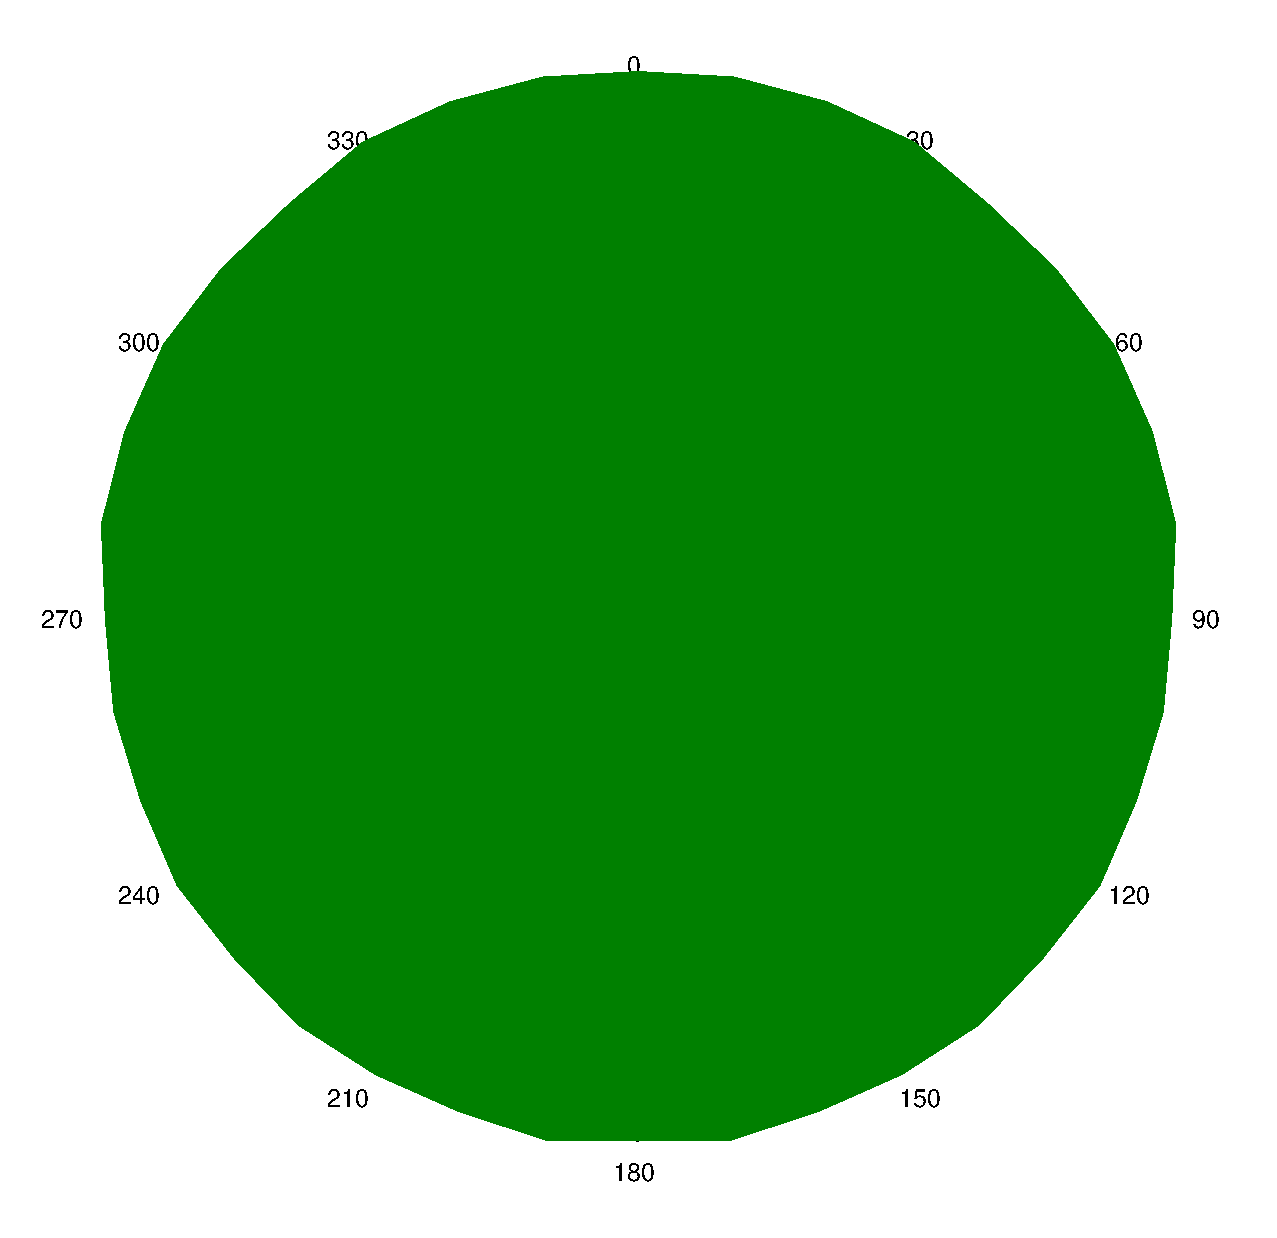
\includegraphics[width=\textwidth]{images/tv3-peak1-angle2.eps}
			\caption{$l = 1, m=0$}
			% \vspace{0.5\baselineskip}
			\label{fig:tv3-1}
		\end{subfigure}
		\begin{subfigure}{0.3\textwidth}
			\centering
			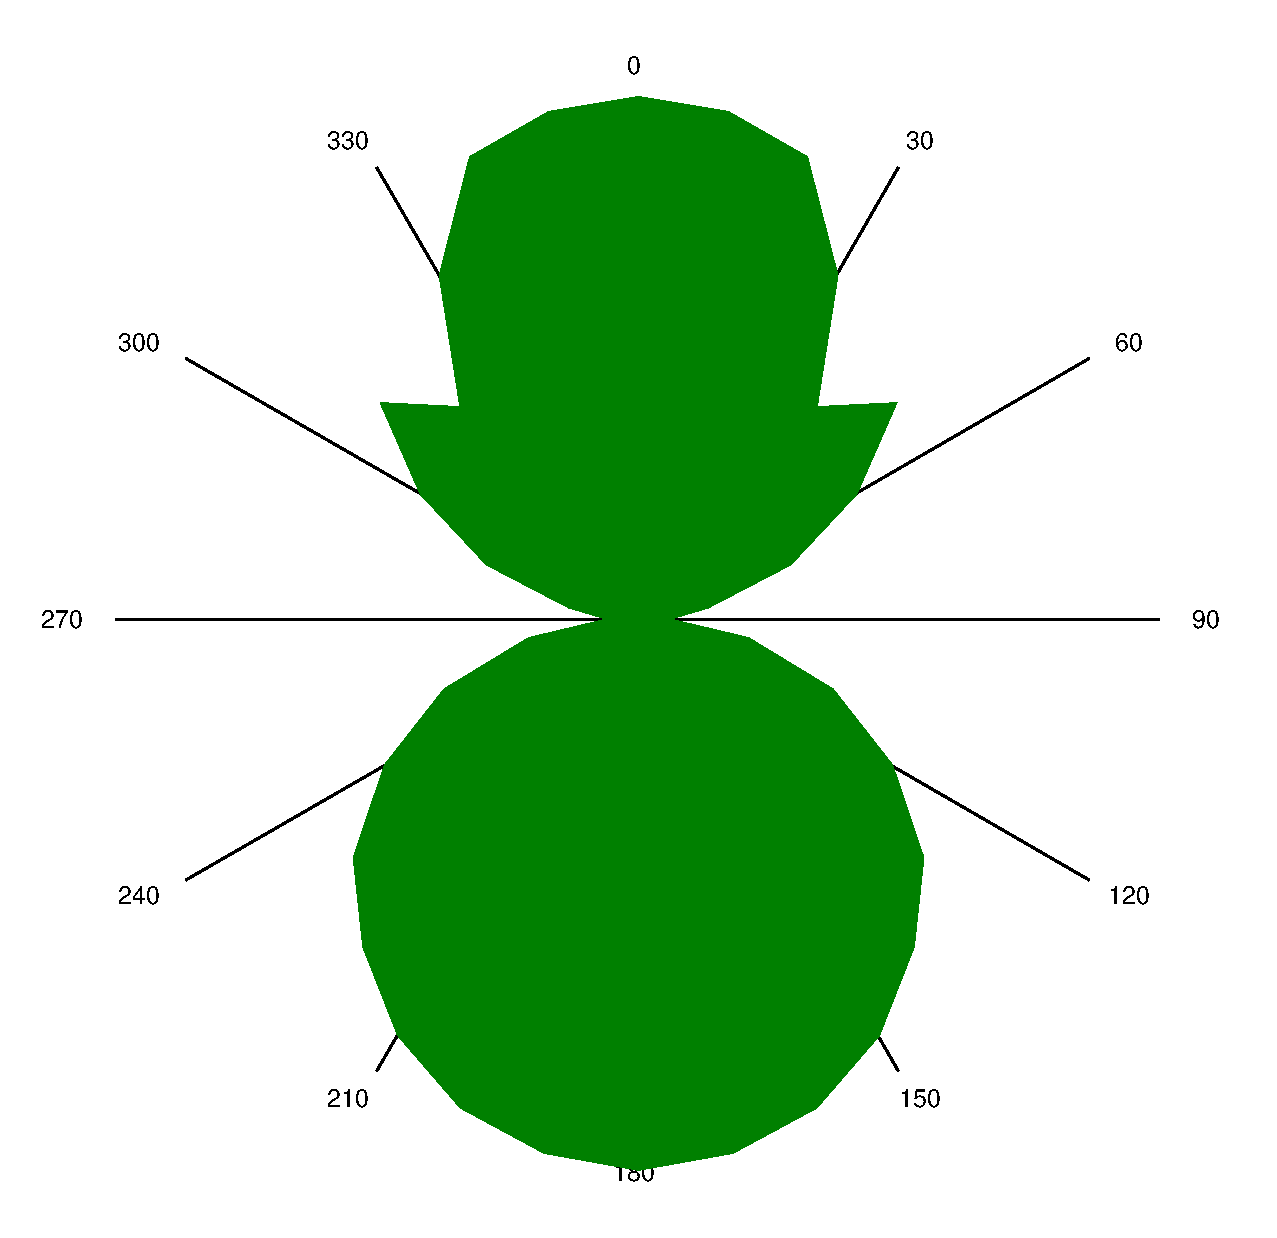
\includegraphics[width=\textwidth]{images/tv3-peak2-angle.eps}
			\caption{$l = 1, m=1$}
			% \vspace{0.5\baselineskip}
			\label{fig:tv3-2}
		\end{subfigure}
		\begin{subfigure}{0.3\textwidth}
			\centering
			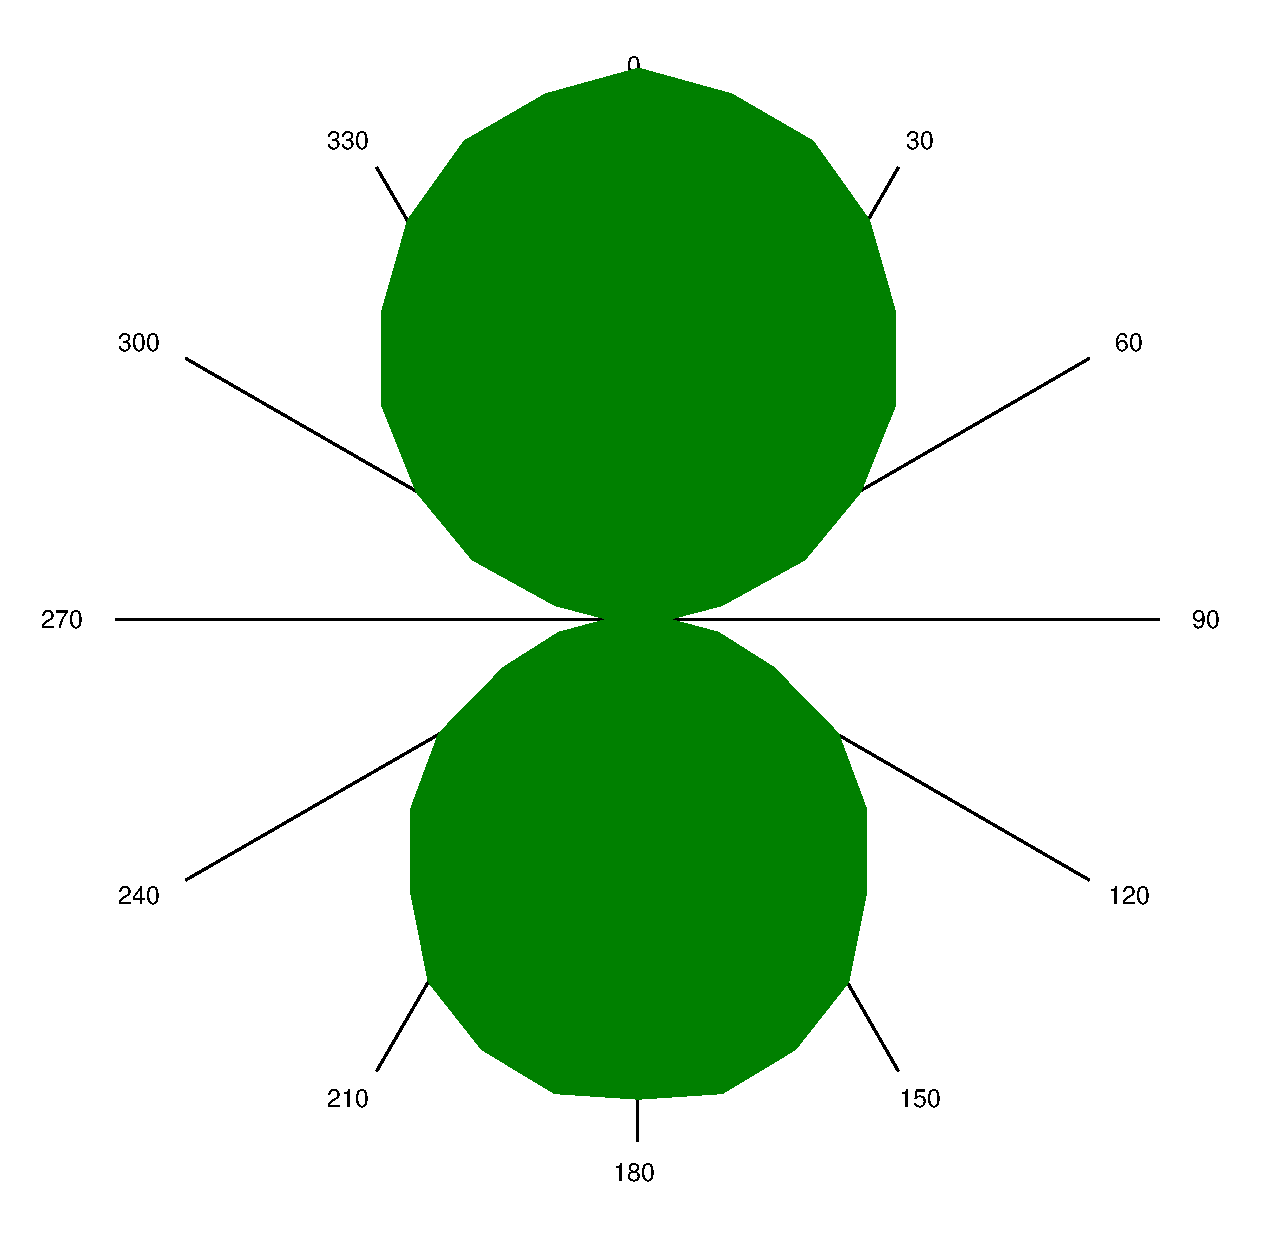
\includegraphics[width=\textwidth]{images/tv3-peak3-angle.eps}
			\caption{$l = 2, m=1$}
			% \vspace{0.5\baselineskip}
			\label{fig:tv3-3}
		\end{subfigure}
		\begin{subfigure}{0.3\textwidth}
			\centering
			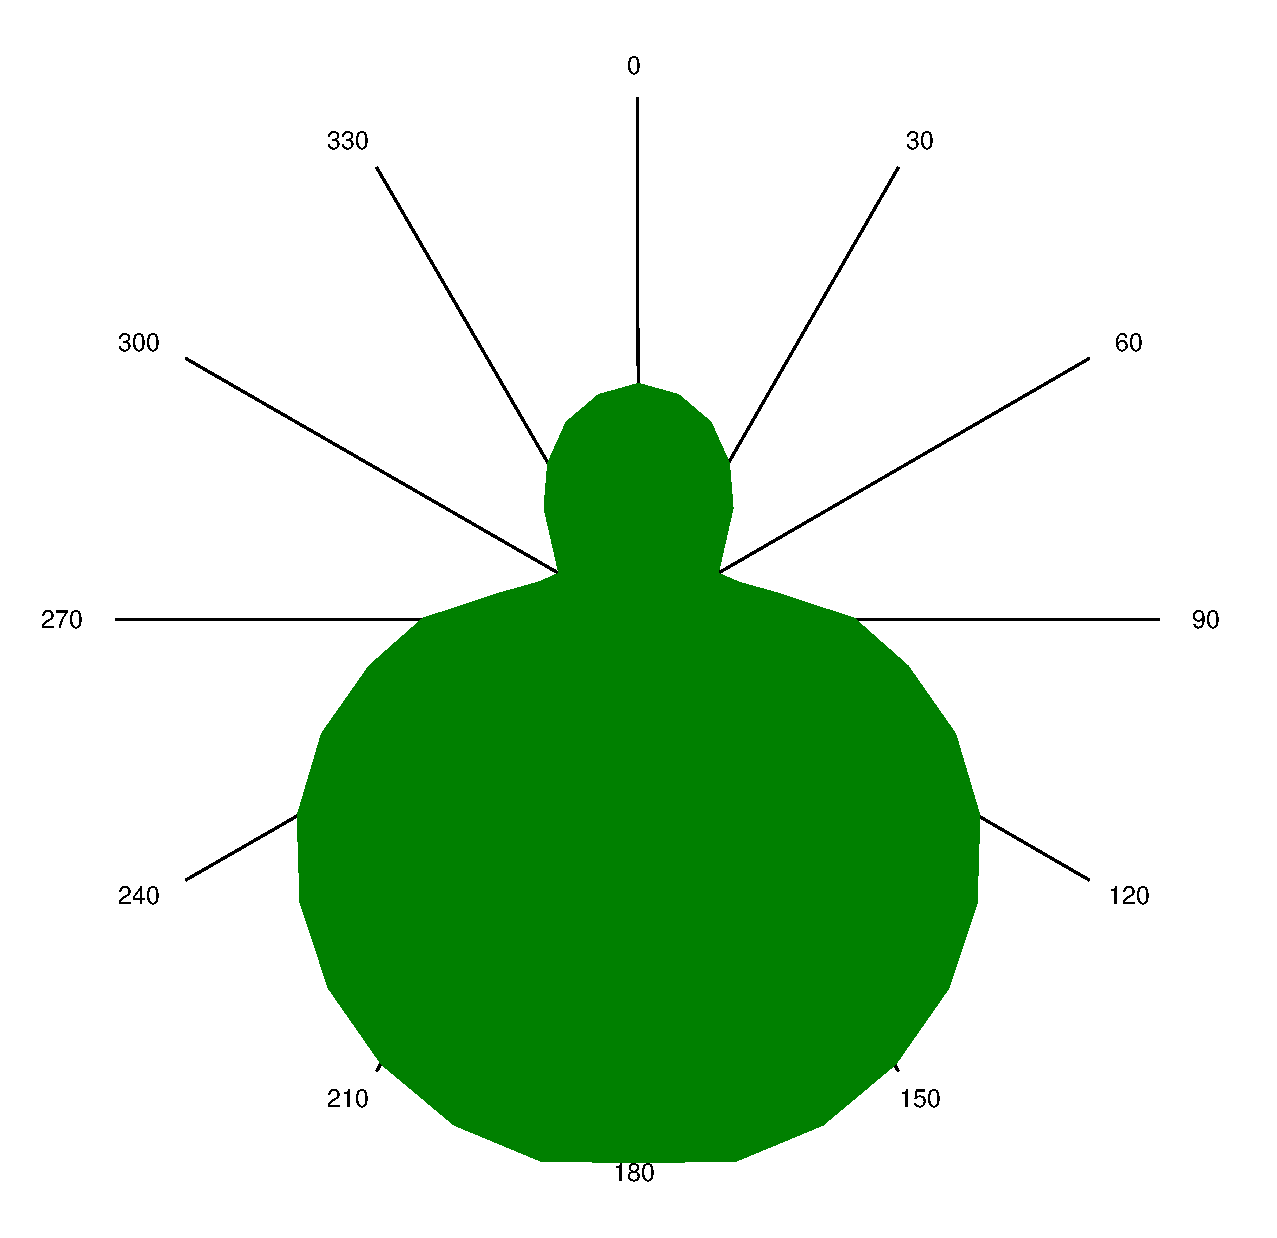
\includegraphics[width=\textwidth]{images/tv3-peak3.5-angle.eps}
			\caption{$l = 2, m=1$?}
			% \vspace{0.5\baselineskip}
			\label{fig:tv3-3.5}
		\end{subfigure}
		\begin{subfigure}{0.3\textwidth}
			\centering
			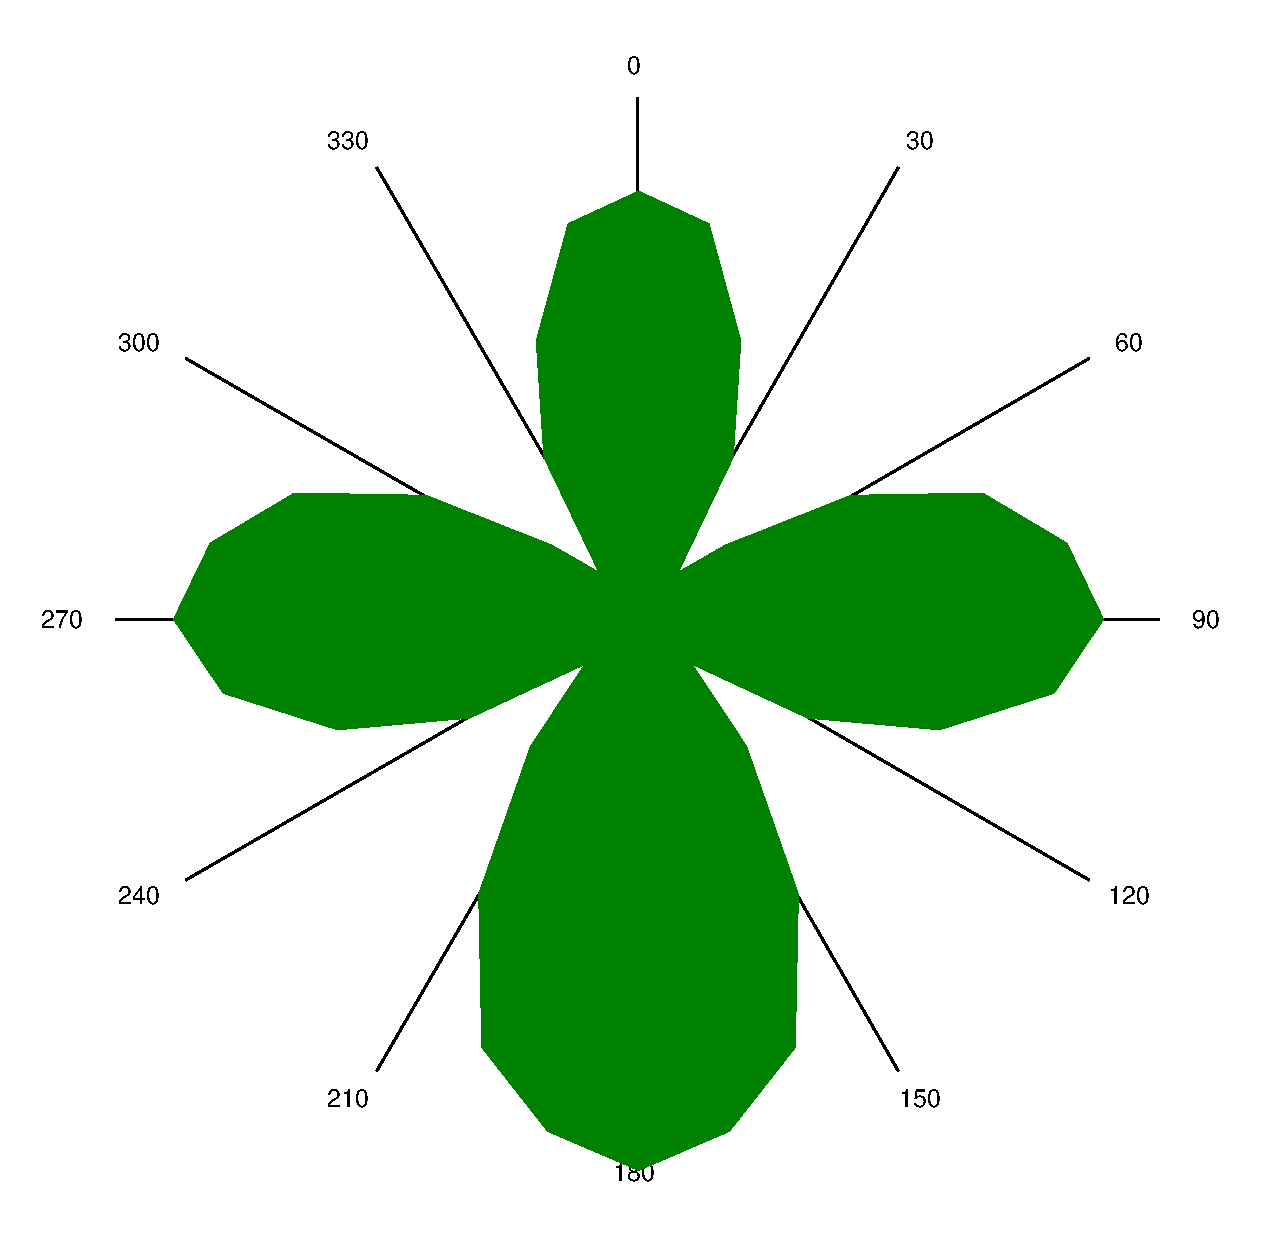
\includegraphics[width=\textwidth]{images/tv3-peak4-angle.eps}
			\caption{$l = 2, m=2$}
			% \vspace{0.5\baselineskip}
			\label{fig:tv3-4}
		\end{subfigure}
	    \caption{Teilversuch 2b}
	\end{figure}

	Die Peak in Abbildung \ref{fig:tv3-3.5} hat wahrscheinlich keine große Bedeutung. Sieht wie ein Übergangszustand aus. Abbildung \ref{fig:tv3-2} ist etwa unsymmetrisch. Der Fehler könnte an Störungen während der Messung liegen, oder der nicht perfekte Resonator.

	Die Abschwächung bei $\varphi = \SI{0}{\degree}$ ist vermutlich der Geomtrie der sphärischen Resonator zufolge. Der Mikrofon liegt direkt oberhalb von der Lautsprecher. Es könnte also sein, dass die Schallwellen schon abgeschwächt ist, wenn sie zurück reflektiert und die Mikrofon erreichen. Wir hören auch während des Versuch was vom Resonator. Die Reflektionen sind also bestimmt nicht perfekt. 

